
\documentclass{article}
\usepackage{amsmath}
\usepackage[utf8]{inputenc}
\usepackage{ctex}
\usepackage{indentfirst}

\usepackage{graphicx}

\usepackage{listings}
\usepackage{color}

\lstset{
    language=Python, % 设置语言
    basicstyle=\ttfamily, % 基本字体样式
    keywordstyle=\color{blue}, % 关键词的颜色
    commentstyle=\color{green}, % 注释的颜色
    stringstyle=\color{red}, % 字符串的颜色
    showstringspaces=false, % 不显示字符串间隙
    numbers=left, % 显示行号
    numberstyle=\tiny\color{gray}, % 行号样式
    breaklines=true, % 自动换行
    frame=single % 给代码框加一个边框
}


\setlength{\parindent}{2em}

\begin{document}

\begin{center}
    \Large \textbf{Lab4 实验报告}\\
    \vspace{1em}
    姓名:陈翎玺~~学号:523030910039~~班级:电院2302
\end{center}

\section{实验概览}

    本次实验主要学习了LSH算法及其在图像匹配加速方面的应用。

    通常,进行图像匹配的时候,我们将图像抽象为一个高维向量,向量的每一维代表其一部分的特征。
    因而,图像匹配的实质便是寻找一张图像,它的特征向量和给定图像的特征向量的距离最近。

    然而,通过暴力枚举数据集中的全部数据,这一过程的复杂度是线性的。
    在给定待匹配的数据集规模极大时,其复杂度是我们不能接受的。
    且当需要匹配的图像数量增多时,复杂度会进一步扩大至平方级别。
    因此,我们需要对其进行优化。常见的优化算法是利用哈希的思想,即本次实验学习的LSH算法。

    LSH算法主要步骤:

    a.将数据映射为一个特定维数向量并实现量化

    b.通过特征向量的Hamming码和对应的取位向量获取相应投影

    c.通过获取投影的种类进行分类实现hash表

    d.对目标图寻找相应的hash项并在对应项中寻找相似图

    类比字符串的Hash算法,如果我们能将图像先进行分类,那么我们只需找到图像所属的类,在类内进行匹配即可。
    理想情况下,图像均匀的落入每一个类中,复杂度因而大大降低。

\section{练习题的解决思路}

\subsection{图像特征向量的计算}

    本次实验中,将图像分为左上、右上、左下、右下四个区域,结合图像的RGB三通道得到12维特征。
    通过各自分量在对应图像中的占比,经过量化函数的映射得到特征。
    此种方法得到的特征维度在本次实验中足以区分图像,但对于规模更大的数据集并不一定可靠,见后文的理论分析。

    为了后续处理的方便,我们选择如下的特征映射函数。

    1. 选取一个数\(C = 2\),作为特征值的最大值,即每个维度的特征值\(p_i \in [0, C] \cap N\)

    2. 根据同一个区域里三种颜色的占比\(p_{ij}\)(由于不区分具体颜色,后文统一记为\(p_j\))
    根据\[
p_i =
\begin{cases}
0, & \text{if } 0 \leq p_j < 0.3 \\
1, & \text{if } 0.3 \leq p_j < 0.6 \\
2, & \text{if } 0.6 \leq p_j
\end{cases}
\]
    计算得到每个维度的特征。这里\(0,1,2\)取决于\(C\)的大小,\(0.3, 0.6\)是给定的超参数,用于划分特征。
    显然,在实际使用中,并不能如ppt当中那样简单粗暴的选取\(0.3, 0.6\)进行分割,需结合选取特征的特点选择。

\subsection{LSH和Hash预处理}

    通过第一步,我们将图像的特征量化,已经可以将其作为根据比较相似度了,但仍然无法解决需要一一匹配的问题。

    类似于字符串哈希中的取模操作,我们选择提取其中几个特征作为代表将其进一步分类。具体如下:

    1.将每一维特征\(p_i\)通过Hamming码展开,得到形如\(111\ldots11100\ldots000\)的数,
    其中1的个数为\(p_i\), 0的个数为\(C - p_i\)。将每一维特征得到的01串简单拼接,得到一个
    长为\(d \times C\)的01串,记为\(v\),这里\(d\)代表数据维数,本实验中为12,具体见前文所述。

    2.选取一个投影集合\(X\),包含若干个元素\(x_i \in [1, d \times C] \cap N\),将\(v\)
    中第\(x_i\)位的数提取并简单拼接,得到投影\(g(p))\)。

    ppt中给出了一种方法。需注意的是ppt中的\(x_i\)指代前文的\(p_i\),同时此做法不利于代码的实现。
    下面给出一种更便于代码实现的方法。

    考虑python代码下标从0开始计数,将选取的\(x_i\)全部减1(也可在给定时按\([0, d \times C]\)
    范围给出),令\(pos = x_i // C\), 如果特征\(p_{pos + 1}\)大于\(x_i \% C\)则投影为1,
    否则为0。主要代码见下,实现中encoder代表特征,由于从0开始计数,pos不需要加1。

\begin{figure}[h]
\centering
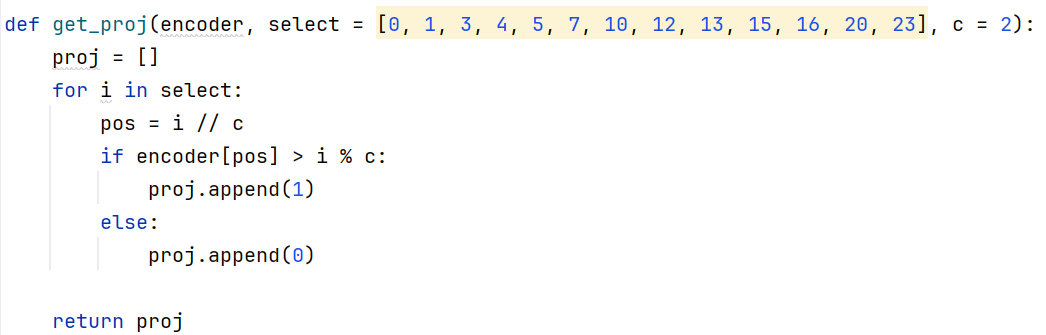
\includegraphics[width=1\textwidth]{./prog_part/1}
\caption{代码片段1}
\end{figure}

\newpage

    g(p)被称作Hash函数,对于容量为N的数据集,g(p)可能的输出有n个,n远小于N,
    这样就将原先的N个数据分成了n个类别,其中每个类别中的数据具有相同的Hash值,
    不同类别的数据具有不同的Hash值。

    对于待检索的输入p,先计算g(p),找到其对应的类别,然后在该类别的数据集中进行搜索,
    速度能够大大加快。主要代码见下:

\begin{figure}[h]
\centering
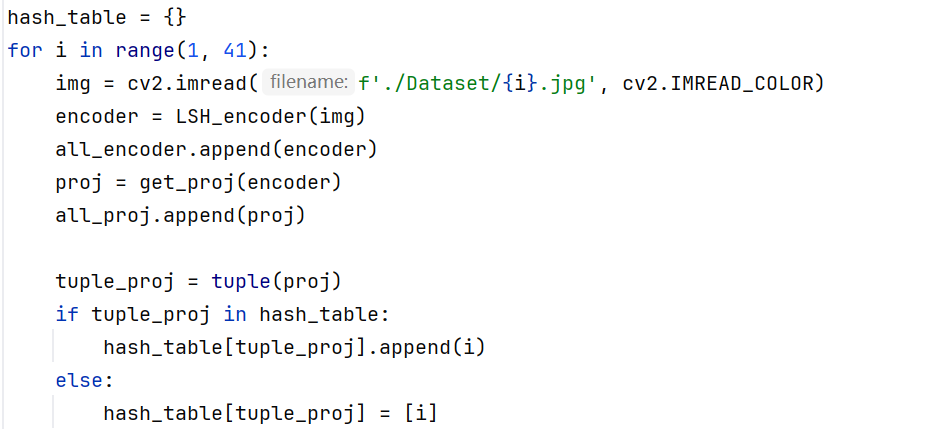
\includegraphics[width=1\textwidth]{./prog_part/2}
\caption{代码片段2}
\end{figure}

    随后可以在类内进行检索。这里简单起见直接使用\(p_i\)的绝对值之差作为判据。如果没有对应的类,
    说明没有和该图像相似程度接近的图像,输出提示即可。

\begin{figure}[h]
\centering
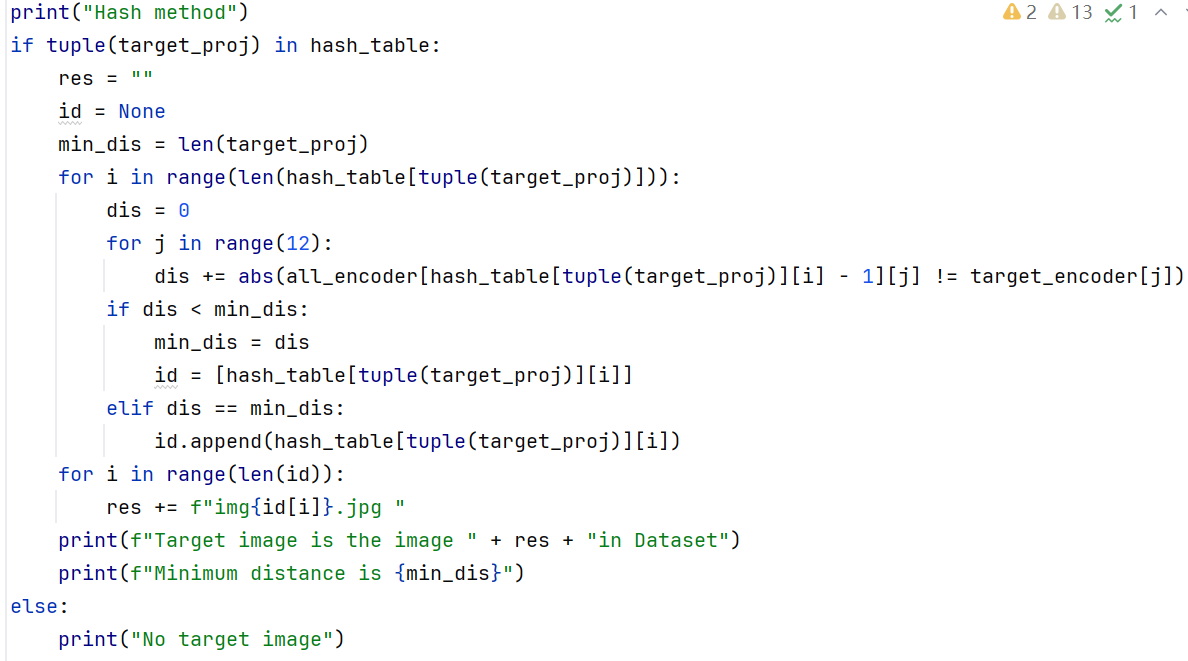
\includegraphics[width=1\textwidth]{./prog_part/3}
\caption{代码片段3}
\end{figure}

\section{代码运行结果}

    以下为完整的代码运行结果,包括Hash method(即LSH)和Knn method(即直接比较)

\begin{figure}[h]
\centering
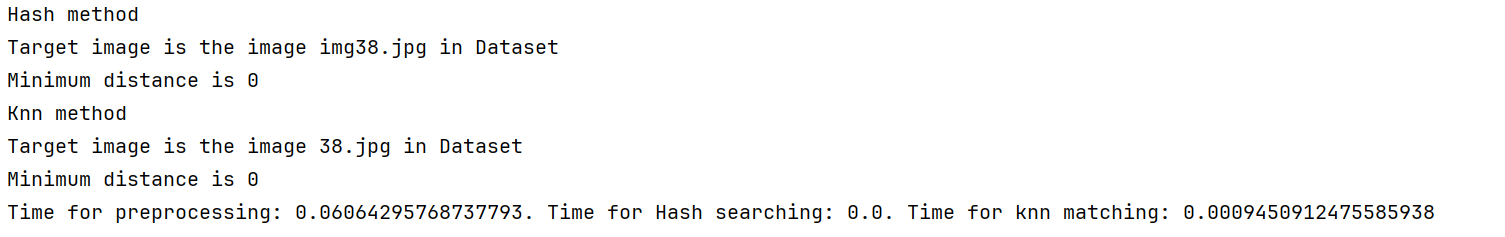
\includegraphics[width=1\textwidth]{./timeHash}
\caption{整体结果}
\end{figure}

\section{实验结果分析与思考}
\subsection{投影集合的选取}

    理论而言,选取n个位置得到投影集合的可能数量为\(2^n\),我们既不希望集合数过少(每个集合当中的图像过多),
    也不希望集合数过多(搜索集合本身的复杂度过大),理想情况下最好使集合数和每个集合的平均图像数相等或接近。

    经测试,由于数据集中存在目标图片,且在\(p_i\)计算公式选取恰当的情况下,总是能唯一确定目标图像,且距离为0.
    但不同的投影集合会生成不同的Hash集合,如选取不当,不利于复杂度的降低,如下图,选择\(0, 4, 9, 11\)作为投影。

\begin{figure}[h]
\centering
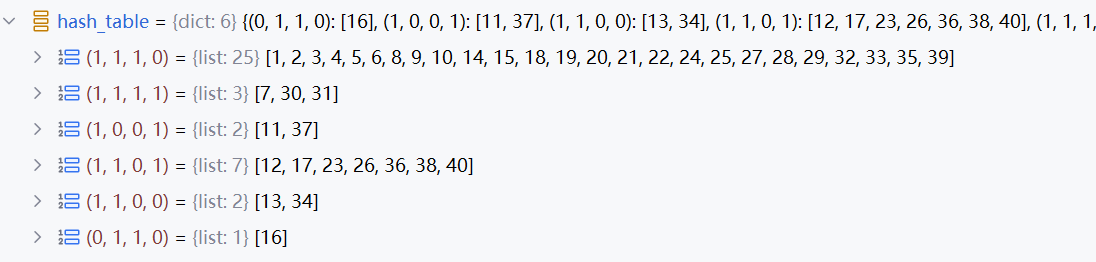
\includegraphics[width=1\textwidth]{./hashtable}
\caption{Hash集合}
\end{figure}

    可以看到,重复的居多,不利于比较。

\subsection{LSH和Knn的效率比较}

    由上文结果和理论分析,Knn的复杂度高于LSH的复杂度。但同时也应注意到,所给的数据集规模小,此时由于运行状态导致的
    时间影响远大于程序本身复杂度的影响,无法较好的比较两者效率。

\subsection{拓展思考回答}

\subsubsection{颜色直方图}

    简单采取\(0.3, 0.6\)的分割效果不尽入人意。简单思考可以发现,由于采用的是占比这一信息,三者并不独立。
    同时,选取的区域过大,对于不明显的特征而言,其占比可能接近。因而,这里选择\(0.2, 0.33\)作为分界,分别反映
    某种颜色是否占比过少或某种颜色是否占据主导来反映特征。就实验结果而言,效果不错。

    检索出的图像和输入图像的相似性体现在特定区域颜色构成上。

\begin{figure}[h]
\centering
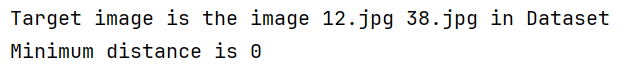
\includegraphics[width=1\textwidth]{./p0306}
\caption{以0.3/0.6为分割的效果图}
\end{figure}

\begin{figure}[h]
\centering
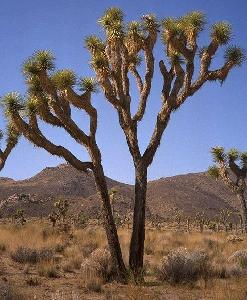
\includegraphics[width=0.4\textwidth]{./Dataset/12}
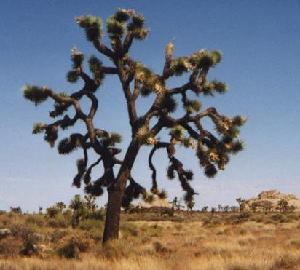
\includegraphics[width=0.4\textwidth]{./Dataset/38}
\caption{img12和img38}
\end{figure}

    上图采用\(0.3, 0.6\)为分割,比较了全部特征值均相等。观察两张图片,发现它们极其相似,
    我们需要更为精确的分割条件。

\section{实验感想}

    本次实验学习了LSH算法,意识到了Hash思想在其他领域的运用。同时明白图像特征的提取和抽象过程,有助于
    图像识别方面的学习。

\section{代码 main.py}
\begin{lstlisting}
import numpy as np
import cv2
import matplotlib.pyplot as plt
import time

def LSH_encoder(img):
    H, W, _ = img.shape
    midpt = [H // 2, W // 2]
    def quant(p):
        if p < 0.2:
            return 0
        elif p < 0.33:
            return 1
        else:
            return 2
    def rgb(image):
        b, g, r = cv2.split(image)
        tot_b = np.sum(b)
        tot_g = np.sum(g)
        tot_r = np.sum(r)
        tot = tot_b + tot_g + tot_r

        p_b = quant(tot_b / tot)
        p_g = quant(tot_g / tot)
        p_r = quant(tot_r / tot)

        return [p_b, p_g, p_r]

    encoder = []
    encoder.extend(rgb(img[:midpt[0], :midpt[1]]))
    encoder.extend(rgb(img[:midpt[0], midpt[1]:]))
    encoder.extend(rgb(img[midpt[0]:, :midpt[1]]))
    encoder.extend(rgb(img[:midpt[0], midpt[1]:]))

    return encoder

def get_proj(encoder, select = [0, 4, 11, 19], c = 2):
    proj = []
    for i in select:
        pos = i // c
        if encoder[pos] > i % c:
            proj.append(1)
        else:
            proj.append(0)

    return proj

st_time = time.time()
target_img = cv2.imread("./target.jpg", cv2.IMREAD_COLOR)
target_encoder = LSH_encoder(target_img)
target_proj = get_proj(target_encoder)

all_encoder = []
all_proj = []

hash_table = {}
for i in range(1, 41):
    img = cv2.imread(f'./Dataset/{i}.jpg', cv2.IMREAD_COLOR)
    encoder = LSH_encoder(img)
    all_encoder.append(encoder)
    proj = get_proj(encoder)
    all_proj.append(proj)

    tuple_proj = tuple(proj)
    if tuple_proj in hash_table:
        hash_table[tuple_proj].append(i)
    else:
        hash_table[tuple_proj] = [i]

min_dis = len(target_proj)
id = None

end_time = time.time()
time1 = end_time - st_time
start_time = time.time()

print("Hash method")
if tuple(target_proj) in hash_table:
    res = ""
    id = None
    min_dis = len(target_proj)
    for i in range(len(hash_table[tuple(target_proj)])):
        dis = 0
        for j in range(12):
            dis += abs(all_encoder[hash_table[tuple(target_proj)][i] - 1][j] != target_encoder[j])
        if dis < min_dis:
            min_dis = dis
            id = [hash_table[tuple(target_proj)][i]]
        elif dis == min_dis:
            id.append(hash_table[tuple(target_proj)][i])
    for i in range(len(id)):
        res += f"img{id[i]}.jpg "
    print(f"Target image is the image " + res + "in Dataset")
    print(f"Minimum distance is {min_dis}")
else:
    print("No target image")

end_time = time.time()
time2 = end_time - start_time
start_time = time.time()

id = None
min_dis = len(target_proj) + 1
for i in range(len(all_proj)):
    dis = 0
    for j in range(len(target_encoder)):
        if all_encoder[i][j] != target_encoder[j]:
            dis += 1
    if dis < min_dis:
        id = [i]
        min_dis = dis
    elif dis == min_dis:
        id.append(i)

res = ""
for i in range(len(id)):
    res += f"{id[i] + 1}.jpg "

end_time = time.time()
time3 = end_time - start_time

print("Knn method")
print(f"Target image is the image " + res + "in Dataset")
print(f"Minimum distance is {min_dis}")

print(f"Time for preprocessing: {time1}. Time for Hash searching: {time2}. Time for knn matching: {time3}")
\end{lstlisting}

\end{document}
